\documentclass[nonacm,sigconf,natbib=false]{acmart}

%%
%% \BibTeX command to typeset BibTeX logo in the docs
\AtBeginDocument{%
  \providecommand\BibTeX{{%
    Bib\TeX}}}

%%
%% The majority of ACM publications use numbered citations and
%% references, obtained by selecting the acmnumeric BibLaTeX style.
%% The acmauthoryear BibLaTeX style switches to the "author year" style.
%%
%% If you are preparing content for an event
%% sponsored by ACM SIGGRAPH, you must use the acmauthoryear style of
%% citations and references.
%%
%% Bibliography style
\RequirePackage[
  datamodel=acmdatamodel,
  style=acmnumeric,
  ]{biblatex}

%% Remove auto generated acm text
\setcopyright{none}
\settopmatter{printacmref=false} % Removes citation information below abstract
\renewcommand\footnotetextcopyrightpermission[1]{} % removes footnote with conference information in first column
\pagestyle{plain}

%% Declare bibliography sources (one \addbibresource command per source)
\addbibresource{linear_agreement_and_liveness.bib}

%%
%% end of the preamble, start of the body of the document source.
\begin{document}

%%
%% The "title" command has an optional parameter,
%% allowing the author to define a "short title" to be used in page headers.
\title{Nebenwirkungen von Optimierungen in Konsensprotokollen} % Original: Linear Agreement and Liveness 

%%
%% The "author" command and its associated commands are used to define
%% the authors and their affiliations.
\author{Eugen Becker}
\email{eugen.becker@fau.de}
\affiliation{%
  \institution{Friedrich-Alexander-Universität Erlangen-Nürnberg}
  \streetaddress{}
  \city{}
  \state{}
  \postcode{}
  \country{}
}

%%
%% By default, the full list of authors will be used in the page
%% headers. Often, this list is too long, and will overlap
%% other information printed in the page headers. This command allows
%% the author to define a more concise list
%% of authors' names for this purpose.
\renewcommand{\shortauthors}{Eugen Becker}

%% Change abstract heading to Kurzfassung
\renewcommand{\abstractname}{Kurzfassung}

%% Change the bibliography title
\renewcommand{\refname}{Literaturverzeichnis}

%%
%% The abstract is a short summary of the work to be presented in the
%% article.
\begin{abstract}
  To do ...

  To do ...

  To do ...

  To do ...

  To do ...

  To do ...

  To do ...

  To do ...

  To do ...

  To do ...

  To do ...

  To do ...
\end{abstract}

%%
%% Keywords. The author(s) should pick words that accurately describe
%% the work being presented. Separate the keywords with commas.
%%\keywords{Do, Not, Us, This, Code, Put, the, Correct, Terms, for,
%%  Your, Paper}

%%
%% This command processes the author and affiliation and title
%% information and builds the first part of the formatted document.
\maketitle

\section{Einleitung}
To do ...

To do ...

To do ...

To do ...

To do ...

To do ...

To do ...

To do ...

To do ...

To do ...

To do ...

To do ...

To do ...

To do ...

To do ...

To do ...

To do ...

To do ...

To do ...

To do ...

To do ...

To do ...

To do ...

To do ...

To do ...

To do ...

To do ...

To do ...

To do ...

To do ...

To do ...

To do ...

To do ...

To do ...

To do ...

To do ...

To do ...

To do ...

To do ...

To do ...
\section{Grundlagen}
In diesem Kapitel wird das grundlegende Wissen vermittelt, das für das Verständnis dieser Arbeit erforderlich ist. Es werden zunächst die Begriffe \emph{State Machine Replication} und \emph{Byzantinische Fehlertoleranz} näher erläutert. Abschließend wird das \emph{System Modell} der Konsensprotokolle beschrieben, die in dieser Arbeit betrachtet werden.

\subsection{State Machine Replication}

Ein bewährter Ansatz, um zuverlässige Dienste zu implementieren, ist State Machine Replication (SMR) \cite{smr-schneider}. Bei diesem Ansatz wird Fehlertoleranz dadurch erreicht, dass ein Dienst als Zustandsmaschine auf mehrere Server repliziert wird, die zusammen ein verteiltes System bilden. Dieses System verhält sich für Clients wie ein einzelner zentraler Dienst, der alle Befehle nacheinander ausführt. Wird der SMR-Ansatz korrekt implementiert, garantiert er die folgenden zwei Eigenschaften \cite{pbft-liveness-problem}:
\begin{itemize}
  \item \textbf{Sicherheit (Safety)}: Alle korrekten Replikate führen dieselbe Abfolge von Clientoperationen auf ihrer Zustandsmaschine aus.
  \item \textbf{Lebendigkeit (Liveness)}: Alle Clientanfragen werden innerhalb einer angemessenen Zeit ausgeführt.
\end{itemize}
Die Implementierung des SMR-Ansatzes gemäß \cite{smr-schneider} setzt deterministische Zustandsmaschinen voraus. Das heißt alle korrekten Replikate starten im selben Zustand und gehen bei gleichen Operationen in den gleichen Zustand über. Um die Sicherheit im SMR-System zu gewährleisten, müssen sich alle korrekten Replikate auf eine einheitliche Reihenfolge einigen, in der sie die Clientanfragen ausführen. Hierzu wird ein Konsensalgorithmus verwendet, der sicherstellt, dass trotz fehlerhafter Replikate eine Einigung (Agreement) erzielt und dem Client geantwortet wird.

In traditionellen SMR-Protokollen existiert ein Anführer-Replikat, das die Reihenfolge der Clientbefehle vorgibt und den Konsensalgorithmus koordiniert. Es gibt aber auch anführerlose Protokolle \cite{smr-leaderless}. Um die Systemlebendigkeit vor fehlerhaften Anführern zu schützen, wird bei anführerbasierten Protokollen zwischen den Modellen \emph{Stable-Leader} und \emph{Leader-Speaks-Once (LSO)} unterschieden \cite{beegees}.
\begin{itemize}
  \item \textbf{Stable-Leader}: Der Anführer wird ausgetauscht, sobald eine Mehrheit korrekter Replikate ihn als fehlerhaft meldet.
  \item \textbf{Leader-Speaks-Once}: Der Anführer wird nach jeder Clientoperation ausgetauscht.
\end{itemize}
Mit jedem Anführerwechsel geht das System in einen neuen Zustand über, der als View bezeichnet wird und als fortlaufende Zahl bzw. als Zähler dargestellt wird. Sinnbildlich kann eine View als Amtszeit eines Anführers gesehen werden.

Es existieren eine Vielzahl unterschiedlicher SMR-Protokolle, die sich in ihrem Konsensalgorithmus und der Art und Weise, wie sie die Lebendigkeit des Systems sicherstellen, unterscheiden.

\subsection{Byzantinische Fehlertoleranz}

In einem verteilten System können verschieden Arten von Fehlern auftreten. Typisch sind dabei zum Beispiel Serverausfälle oder Kommunikationsfehler, die durch Netzwerkprobleme verursacht werden. Bei Fail-Stop-Fehlern geht ein Replikat, bevor es aufgrund eines Fehlers stoppt, in einen Zustand über, der den anderen Replikaten signalisiert, dass ein Fehler aufgetreten ist. Ein Server kann aber auch bei einem Crash-Fehler in einem willkürlichen Zustand stoppen. Bei Kommunikationsfehlern können Nachrichten aufgrund von Netzwerkproblemen verloren gehen, verzögert werden oder in falscher Reihenfolge eintreffen. Allgemein gilt ein Replikat im Kontext von State Machine Replication als fehlerhaft, wenn es sich nicht gemäß den Spezifikationen im Protokoll verhält \cite{smr-schneider}.

Eine besondere Herausforderung stellen Byzantinische-Fehler dar, bei denen sich ein Replikat willkürlich oder bösartig gegenüber anderen Replikaten oder dem Client verhalten kann \cite{smr-schneider}. Sie sind schwer zu ermitteln, weil byzantinisch fehlerhafte Replikate nicht immer als fehlerhaft wahrgenommen werden. Beispiele hierfür sind: (1) Absichtliches Versenden falscher oder widersprüchlicher Informationen; (2) Absichtliches Verzögern oder Auslassen von Nachrichten; (3) Gezielte Irreführung ausgewählter Komponenten (andere Replikate und/oder Clients) bei gleichzeitig korrektem Verhalten gegenüber den übrigen Komponenten; praktisch jedes willkürliche Verhalten ist denkbar. Byzantinische Fehler können durch verschiedene Faktoren verursacht werden, wie zum Beispiel Softwarefehler, Hardwareausfälle, Netzwerkprobleme oder böswillige Angriffe.

Der Begriff Byzantinischer-Fehler hat seinen Ursprung im Paper "The Byzantine Generals Problem"\cite{byzantine-generals-problem} von Lamport et al. In einer Analogie beschreiben die Autoren, dass eine Einigung über die nächste Clientoperation in SMR-Systemen trotz Byzantinischer-Fehler zustande kommen kann, wenn das System aus mindestens $3f+1$ Replikaten besteht, wobei $f$ für die Anzahl fehlerhafter Replikate steht. Das liegt daran, dass für jeden Vorschlag des Anführers sichergestellt werden muss, dass eine Mehrheit korrekter Replikate abstimmt. Diese Mehrheit ist gegeben, wenn für jede Abstimmung ein Quorum aus $2f+1$ Replikaten abstimmt. Da aber auch korrekte Replikate unter Umständen nicht rechtzeitig antworten können, werden insgesamt $3f+1$ Replikate benötigt (siehe Abbildung ).

SMR-Protokolle, die Byzantinische-Fehler tolerieren können werden als \emph{Byzantine Fault Tolerant State Machine Replication (BFT-SMR)} bezeichnet.

\begin{figure}
  \centering
  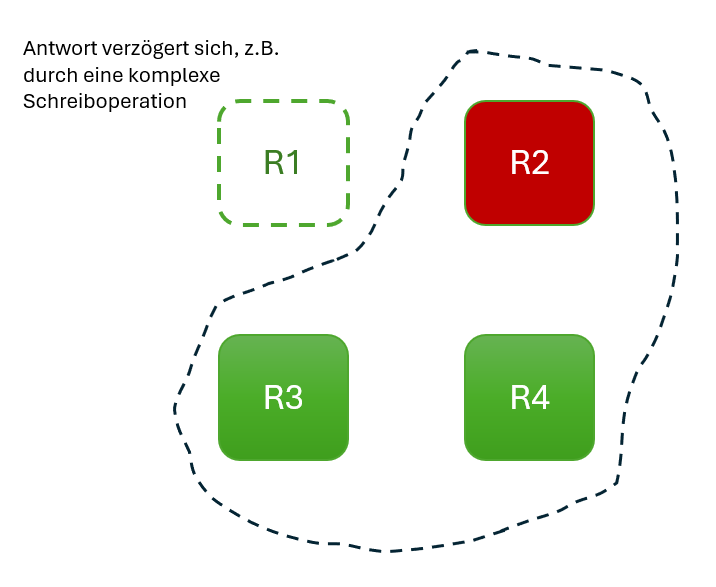
\includegraphics[width=0.5\linewidth]{bft-quorum.png}
  \caption{To Do: Notwendigkeit für 3f+1 Replikate}
  \Description{To Do}
  \label{fig:bft-quorum}
\end{figure}

\subsection{System Modell}

To Do

\section{Nebenwirkungen durch Optimierungen in PBFT und HotStuff}

In diesem Kapitel werden etablierte Optimierungen in den BFT-SMR-Protokollen Practical Byzantine Fault Tolerance und HotStuff vorgestellt, die unter bestimmten Bedingungen die Systemlebendigkeit beeinträchtigen können. Zunächst wird zu jedem Protokoll der Konsensalgorithmus beschrieben, gefolgt von einer Optimierung, die die Effizienz des Algorithmus steigert. Es werden die möglichen Nebenwirkungen dieser Optimierungen aufgezeigt und abschließend Lösungen präsentiert, um diese Nebenwirkungen zu umgehen.

\subsection{Practical Byzantine Fault Tolerance}

Practical Byzantine Fault Tolerance (PBFT)\cite{pbft} von Castro und Liskov war das erste BFT-SMR-Protokoll, dass in einem partiell synchronen Netzwerk effizient genug war, um in der Praxis eingesetzt werden zu können. Auf den Design-Entscheidungen von PBFT basieren viele BFT-SMR-Protokolle, die weitere Verbesserungen vorgenommen haben, z.B. Zyzzyva\cite{zyzzyva}, Aardvark\cite{aardvark} und BFT-SMaRt\cite{bft-smart}. PBFT ist ein anführerbasiertes Protokoll, das das Stable-Leader Modell implementiert, das heißt neben dem Konsensalgorithmus gibt es einen separaten Algorithmus für den Anführerwechsel. Alle Replikate ohne Anführerrolle werden als Backup bezeichnet.

\subsubsection{PBFT-Konsensalgorithmus}

Der Konsensalgorithmus von PBFT besteht aus den Phasen \emph{Pre-prepare}, \emph{Prepare} und \emph{Commit} (siehe Abbildung \ref{fig:pbft-normal}). Er beginnt damit, dass ein Client seine Anfrage an alle Replikate im verteilten System sendet.

\textbf{Pre-Prepare-Phase.} Sobald das Anführer-Replikat die Nachricht des Clients erhalten und auf ihre Gültigkeit überprüft hat, vergibt es der Nachricht eine Sequenznummer. Diese bestimmt die Reihenfolge, in der die Clientoperation auf allen Replikaten ausgeführt werden soll. Anschließend erstellt es eine Pre-Prepare-Nachricht, bestehend aus der Clientoperation, der Sequenznummer und der aktuellen View. Diese Nachricht wird signiert und an alle Backups im System verteilt.

\textbf{Prepare-Phase.} Alle Backups stimmen darüber ab, ob die vom Anführer vorgeschlagene Clientoperation ausgeführt werden soll. Hierzu überprüft jedes Backup die Pre-Prepare-Nachricht auf ihre Gültigkeit und auf mögliche Konflikte mit ihrem aktuellen Zustand und der ursprünglichen Nachricht des Clients. Hat ein Backup die Pre-Prepare-Nachricht akzeptiert, gibt es ihre Stimme ab, indem es eine Prepare-Nachricht an alle anderen Replikate (einschließlich des Anführers) sendet. Jedes Replikat sammelt $2f$ gültige Prepare-Nachrichten von unterschiedlichen Replikaten (einschließlich seiner eigenen, falls vorhanden). Zusammen mit der Pre-Prepare-Nachricht des Anführers ergibt das ein Quorum von $2f+1$ Stimmen.

\textbf{Commit-Phase.} Hat ein Replikat (egal ob Anführer oder Backup) ein Prepare-Quorum erreicht, signalisiert es dies, indem es eine Commit-Nachricht an alle anderen Replikate sendet. Jedes Replikat sammelt ein Quorum von $2f+1$ gültigen Commit-Nachrichten von unterschiedlichen Replikaten (einschließlich seiner eigenen, falls vorhanden). Hat es ein Commit-Quorum erreicht, bedeutet es, dass eine Einigung erfolgt ist. Das Replikat schreibt die Clientoperation fest (commit) und führt diese anschließend auf seiner Zustandsmaschine aus. Zum Schluss wird das Ergebnis an den Client gesendet.

Ein Client wartet auf $f+1$ übereinstimmende Antworten von unterschiedlichen Replikaten, bevor er die Antwort akzeptiert.

\begin{figure}
  \centering
  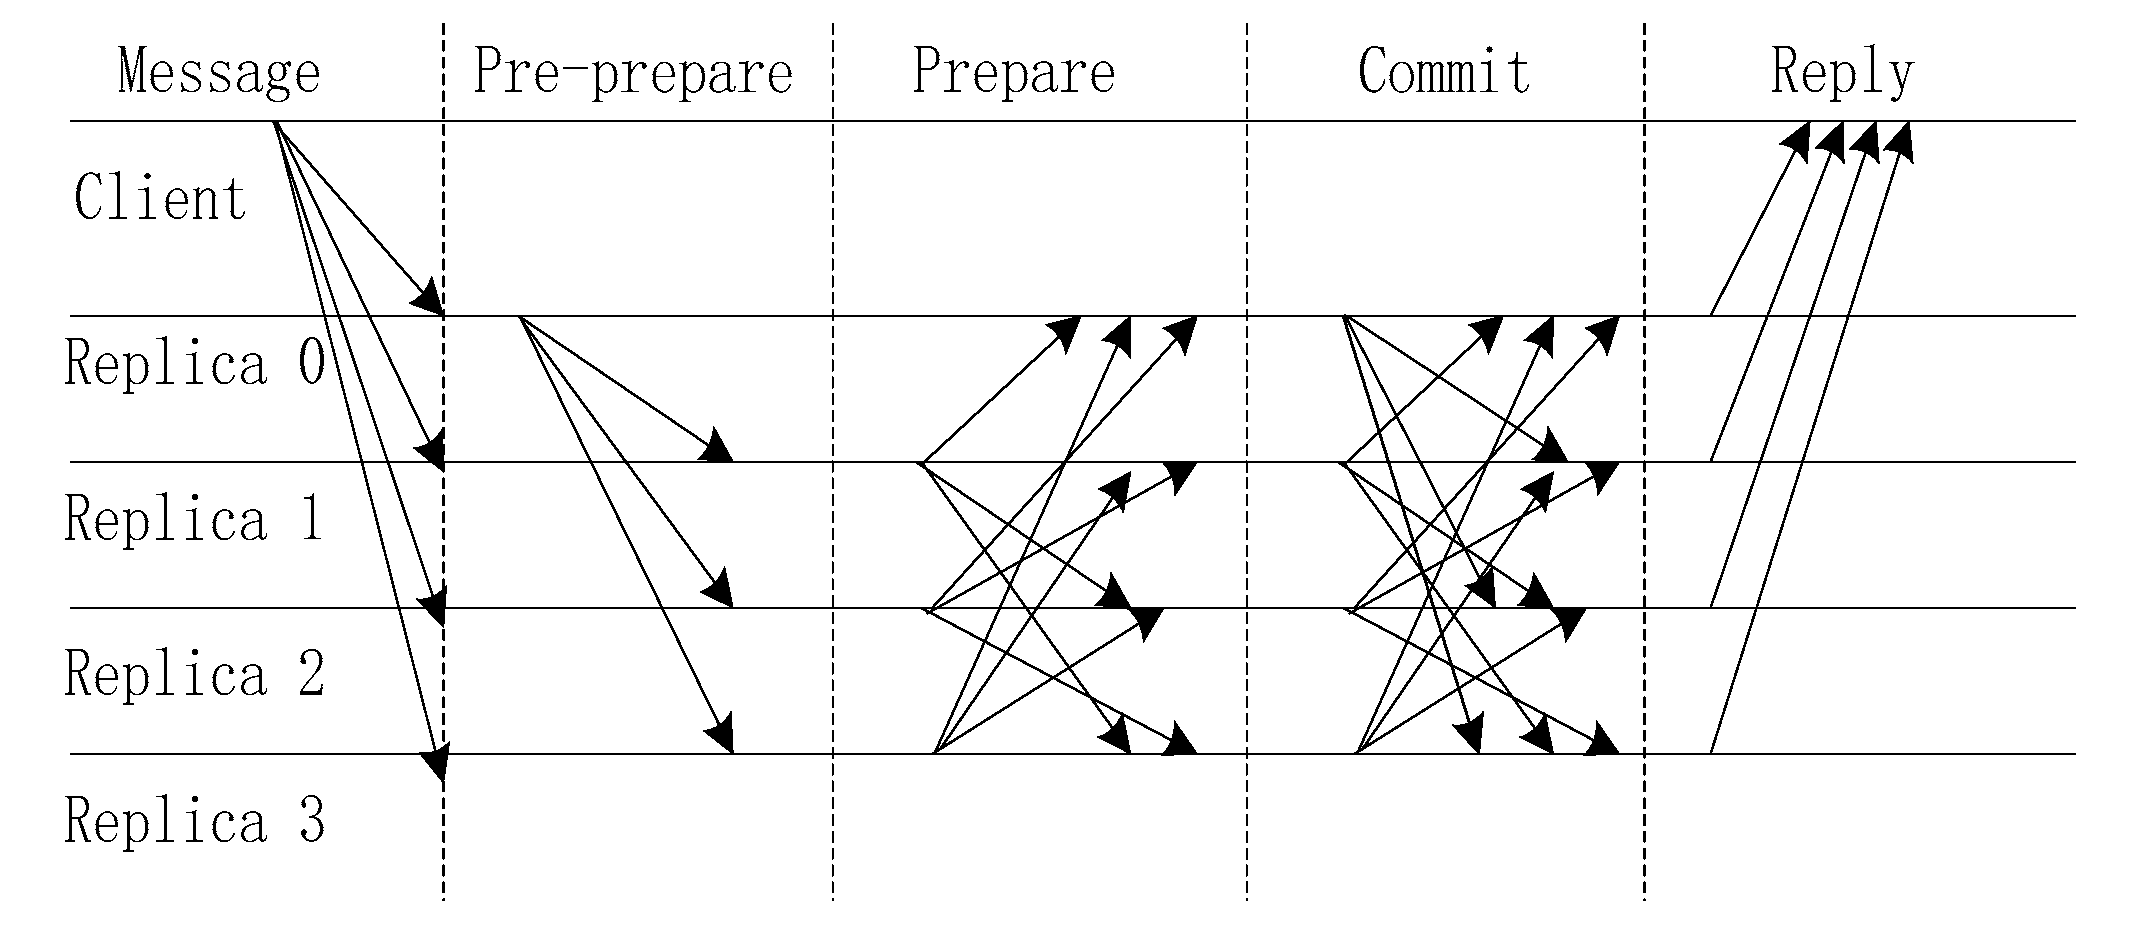
\includegraphics[width=\linewidth]{pbft-normal.png}
  \caption{PBFT-Konsensalgorithmus im fehlerfreien Fall}
  \Description{PBFT-Konsensalgorithmus im fehlerfreien Fall}
  \label{fig:pbft-normal}
\end{figure}

\subsubsection{Read-Only Optimierung}

Der Konsensalgorithmus von PBFT hat eine hohe Nachrichtenkomplexität von $O(n^2)$. Deshalb haben die Autoren von PBFT mehrere Optimierungen vorgestellt, die das Protokoll effizienter machen sollen \cite{pbft-optimization}. Eine davon ist die Read-Only Optimierung. Sie erlaubt es Leseanfragen ohne Durchlauf des Konsensalgorithmus beantworten zu dürfen. Die Überlegung hierbei ist, dass Leseoperationen den Zustand des Systems nicht verändern und deshalb sofort ausgeführt werden können. Die Read-Only Optimierung setzt allerdings zwei Bedingungen voraus:
\begin{enumerate}
  \item Ein Replikat muss alle vorherigen Operationen festgeschrieben haben (commit), bevor es eine Read-Only-Anfrage ausführen darf.
  \item Der Client muss bei allen Anfragen (Lesen und Schreiben) auf $2f+1$ übereinstimmende Antworten von unterschiedlichen Replikaten warten, bevor er das Ergebnis akzeptiert, unabhängig davon, ob der Konsensalgorithmus durchlaufen wurde oder nicht. 
\end{enumerate}
Abbildung \ref{fig:pbft-optimization} zeigt, dass ein Client, der wie im nicht-optimierten Fall ein Ergebnis aus $f+1$ Antworten akzeptiert, Gefahr läuft, einen veralteten Stand zu lesen. Das liegt daran, dass korrekte Replikate mit der Ausführung festgeschriebener Clientoperationen zurückliegen können und mit einem alten Ergebnis antworten (siehe Abbildung \ref{fig:pbft-optimization links}). Zusätzlich kann eine Kombination aus byzantinisch fehlerhaften Replikaten, die absichtlich ein altes Ergebnis liefern, und zurückliegenden korrekten Replikaten dazu führen, dass ein Client trotz $2f+1$ identischer Antworten einen veralteten Stand liest (siehe Abbildung \ref{fig:pbft-optimization rechts}). Deshalb ist Bedingung (2) auch bei Schreibanfragen notwendig, obwohl diese den Konsensalgorithmus durchlaufen. Wenn ein Client nicht genügend übereinstimmende Antworten erhalten hat, wiederholt er die Leseanfrage als Read-Write-Anfrage, die den Konsensalgorithmus durchlaufen muss.

\begin{figure}
  \centering
  \includegraphics[width=\linewidth]{pbft_read_quorum_erklärung.png}
  \caption{Grund}
  \Description{Grund}
  \label{fig:pbft-optimization}
\end{figure}

\subsubsection{Angriff auf Read-Only Optimierung}

Die Bedingung, dass ein Client bei allen Anfragen auf $2f+1$ übereinstimmende Antworten von unterschiedlichen Replikaten warten muss, bevor er ein Ergebnis akzeptieren darf, kann bei einem bestimmten Angriff dazu führen, dass das gesamte System blockiert wird \cite{pbft-liveness-problem}. Dieser Angriff beinhaltet $f$ byzantinisch fehlerhafte Replikate, darunter den Anfüher und zielt darauf ab, dass kein Client genügend übereinstimmende Antworten sammeln kann, um ein Ergebnis zu akzeptieren.

Im Detail verläuft der Angriff wie folgt (siehe Abbildung \ref{fig:read-only-problem}): Nach Erhalt einer Schreibanfrage, isoliert der fehlerhafte Anführer $f$ korrekte Backups, indem er ihnen keine Pre-Prepare-Nachricht sendet. Den restlichen Backups verhält er sich dem Protokoll entsprechend richtig. Alle nicht-isolierten Backups und der Anführer durchlaufen anschließend die Prepare- und Commit-Phase. Währenddessen ignorieren die isolierten Backups alle Prepare- und Commit-Nachrichten, weil sie keine zugehörige Pre-Prepare-Nachricht in ihrem Log haben. Am Ende der Commit-Phase führen alle nicht-isolierten Backups und der Anführer die Clientoperation aus, allerdings antwortet der Anführer dem Client absichtlich nicht. Das sorgt dafür, dass der Client maximal $2f$ Antworten erhält (maximal, weil außer dem Anführer noch andere Replikate fehlerhaft sein können). Aufgrund der Read-Only Optimierung benötigt der Client aber $2f+1$ Antworten, um ein Ergebnis zu akzeptieren. Infolgedessen wiederholt er seine Anfrage, was aber wieder zum gleichen Ergebnis führt.

Um den böswilligen Anführer zu wechseln, muss ein View-Wechsel durchgeführt werden. In PBFT löst jedes korrekte Backup, das einen fehlerhaften Anführer bemerkt hat, eine View-Change-Nachricht aus. Bei $2f+1$ View-Change-Nachrichten wird der Anführer gewechselt. Dieses Quorum ist notwendig, damit keine fehlerhaften Backups absichtlich View-Wechsel auslösen können. Bei diesem Angriff kommt es aber zu keinem Anführerwechsel, weil die benötigte Anzahl an View-Change-Nachrichten nicht erreicht wird. Diese werden nämlich nur von den $f$ isolierten Backups ausgelöst, weil sich der Anführer nur diesen fehlerhaft gegenüber verhält. Als Resultat dieses Angriffs kann das System keinen Fortschritt mehr machen, was eine Verletzung der Liveness-Garantie darstellt.

\begin{figure}
  \centering
  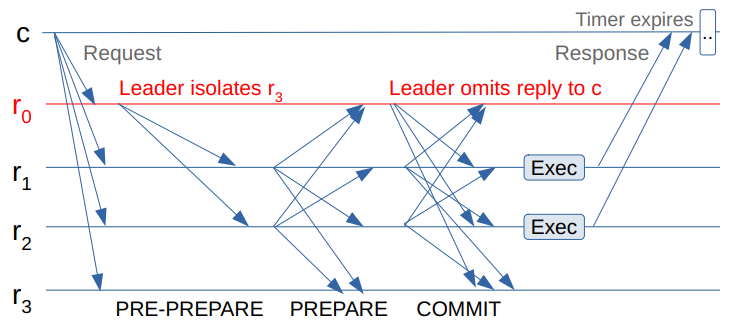
\includegraphics[width=\linewidth]{read-only-problem.png}
  \caption{Grund}
  \Description{Grund}
  \label{fig:read-only-problem}
\end{figure}

\subsubsection{Lösung für Read-Only Optimierungsproblem}

Um den Angriff auf die Read-Only Optimierung wirkungslos zu machen, muss sichergestellt werden, dass der Client ein Quorum von übereinstimmenden Antworten erhält. Hierzu wird der Konsensalgorithmus um eine weitere Phase ergänzt (siehe Abbildung \ref{read-only-korrektur}). Nachdem ein Replikat ein Quorum von Commit-Nachrichten gesammelt (Konsensentscheidung erreicht) und die neue Clientoperation festgeschrieben hat, sendet es eine Forward-Decision-Nachricht an alle Replikate. Diese Nachricht enthält 2f+1 Commit-Nachrichten als Nachweis dafür, dass ein Konsens erreicht wurde. Sobald ein isoliertes Replikat eine gültige Forward-Decision-Nachricht erhalten hat, kann es die neue Clientoperation auf seiner Zustandsmschine ausführen und dem Client antworten. Auf diese Weise kann ein korrektes Replikat eine neue Clientoperation festschreiben, sobald es ein Quorum von Commit-Nachrichten gesammelt oder durch eine Forward-Decision-Nachricht erhalten hat.

\begin{figure}
  \centering
  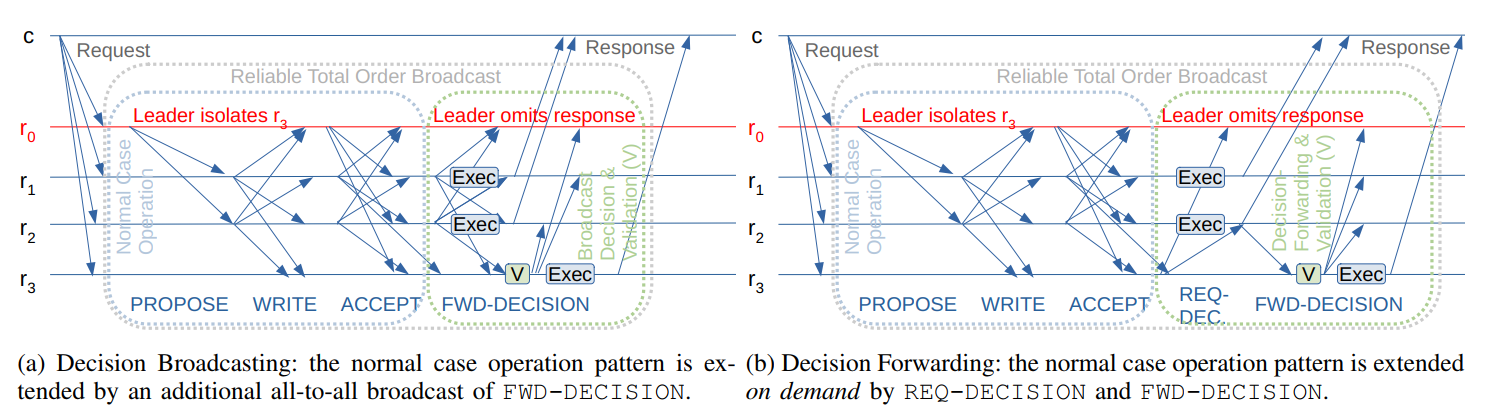
\includegraphics[width=\linewidth]{read-only-korrektur.png}
  \caption{Grund}
  \Description{Grund}
  \label{fig:read-only-korrektur}
\end{figure}

\subsection{HotStuff}

HotStuff\cite{hotstuff} wurde entwickelt, um ein einfaches BFT-SMR-Protokoll bereitzustellen, das hohe Skalierbarkeit bietet. Im Gegensatz zu PBFT, wo jedes Replikat ein Quorum aus signierten Nachrichten unterschiedlicher Replikate sammeln muss, übernimmt bei HotStuff nur der Anführer diese Aufgabe. Aus den Nachrichten der Replikate erstellt der Anführer ein Quorum-Zertifikat (QZ). Ein QZ ist ein Nachweis dafür, dass während einer bestimmten Phase des Konsensalgorithmus ein Quorum von $2f+1$ Replikaten für eine Clientoperation gestimmt haben. In HotStuff werden Clientbefehle in Blöcken gespeichert. Jeder Block enthält einen Clientbefehl sowie eine Referenz auf seinen Vorgängerblock. Dadurch entsteht eine geordnete Kette von Clientoperationen, die auf allen Zustandsmaschinen ausgeführt werden. Jedes Quorum-Zertifikat enthält einen zugehörigen Block, mit Clientoperation. HotStuff ist ein anführerbasiertes Protokoll, das das Leader-Speaks-Once Modell implementiert, das heißt nach jeder Clientoperation wird der Anführer gewechselt.

\subsubsection{HotStuff-Konsensalgorithmus}

Der Konsensalgorithmus von HotStuff besteht aus den Phasen \emph{prepare}, \emph{pre-commit}, \emph{commit} und \emph{decide} (siehe Abbildung \ref{fig:hotstuff}). Zu Beginn jeder Prepare-Phase findet ein View-Wechsel statt, wodurch jeder Durchlauf mit einem neuen Anführer startet.

\textbf{Prepare-Phase.} Das neue Anführer-Replikat bekommt von allen anderen Replikaten New-View-Nachrichten geschickt, aus denen es das höchste bekannte Prepare-QZ im System ermittelt. Dieses wird als High-QZ bezeichnet und enthält den aktuellsten Block der Kette an Clientoperationen. Sobald der Anführer eine neue Clientanfrage erhält, erstellt er einen neuen Block mit dieser Anfrage und setzt den Block aus High-QZ als Vorgänger. Anschließend verschickt er eine Prepare-Nachricht an alle Replikate, bestehend aus der aktuellen View, dem neuen Block als Vorschlag und High-QZ als Nachweis für das Zustandekommen eines Quorums. Jedes Replikat überprüft die Nachricht auf ihre Gültigkeit und akzeptiert den neuen Block, wenn er eine logische Erweiterung der Kette an Clientoperationen darstellt. Hat ein Replikat die Prepare-Nachricht akzeptiert, gibt es seine Stimme ab, indem es eine Prepare-Vote-Nachricht an den Anführer sendet.

\textbf{Pre-Commit-Phase.} Der Anführer sammelt ein Quorum von $2f+1$ Prepare-Vote-Nachrichten und kombiniert diese zu einem Prepare-QZ. Anschließend verschickt er eine Pre-Commit-Nachricht mit dem Prepare-QZ an alle Replikate. Diese antworten mit einer Pre-Commit-Vote-Nachricht.

\textbf{Commit-Phase.} Wenn der Anführer ein Quorum von Pre-Commit-Vote-Nachrichten erhalten hat, kombiniert er diese zu einem Pre-Commit-QZ und verschickt es in einer Commit-Nachricht an alle Replikate. Diese antworten mit einer Commit-Vote-Nachricht. In dieser Phase sperrt ein Replikat seinen Zustand auf dem vorgeschlagenen Block. Das heißt es akzeptiert nur noch einen neuen Block, wenn er den aktuell gesperrten Block als Vorgänger hat oder sich in einer höheren View befindet als dieser. Das ist notwendig, damit keine widersprüchlichen Clientoperationen akzeptiert werden können (Sicherheitsgarantie).

\textbf{Decide-Phase.} Sobald der Anführer ein Quorum von Commit-Vote-Nachrichten gesammelt hat, kombiniert er diese zu einem Commit-QZ und verschickt es in einer Decide-Nachricht an alle Replikate. Durch die Decide-Nachricht weiß ein Replikat, dass der vorgeschlagene Knoten bzw. Clientbefehl festgeschrieben und auf der Zustandsmaschine ausgeführt werden darf. Nachdem es die Operation ausgeführt und eine Antwort an den Client gesendet hat, erhöht es den View-Zähler und startet eine neue View durch das Versenden einer New-View-Nachricht an den neuen Anführer.

Ebenso wie in PBFT wartet der Client auf $f+1$ identische Antworten von unterschiedlichen Replikaten, bis er eine Antwort akzeptiert.

\begin{figure}
  \centering
  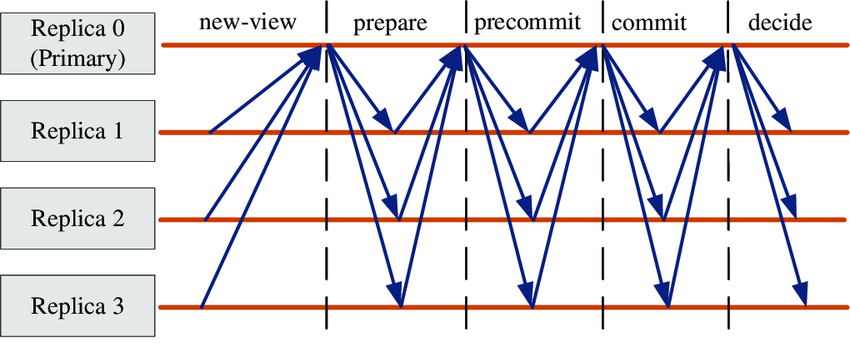
\includegraphics[width=\linewidth]{hotstuff.png}
  \caption{Grund}
  \Description{Grund}
  \label{fig:hotstuff}
\end{figure}

\subsubsection{Chained HotStuff}

Betrachtet man die einzelnen Phasen von HotStuff, so fällt auf, dass sie sich sehr ähneln. In jeder Phase sammelt der Anführer genügend Vote-Nachrichten, um ein Quorum-Zertifikat zu bilden. Die Autoren von HotStuff machen sich diese Eigenschaft zunutze und vereinfachen den Konsensalgorithmus. Die Idee ist, dass nach jeder Prepare-Phase ein View-Wechsel stattfindet und eine neue Clientoperation vorgeschlagen wird. Einzelne Phasen überlappen sich und werden parallel ausgeführt, indem sie ein gemeinsames Quorum-Zertifikat (Generic-QZ) als Nachweis nutzen. Dadurch entsteht eine Art Pipeline, was den Durchsatz erhöht. Diese Optimierung wird Chained HotStuff genannt und funktioniert wie folgt (siehe Abbildung \ref{chained-hotstuff}):

Jede Prepare-Phase beginnt damit, dass der neue Anführer von View $v$ ein Generic-QZ vom vorherigen Anführer erhält. Er erstellt einen neuen Block $b$ mit einer neuen Clientoperation $cmd_1$ und sendet diesen samt Generic-QZ als Vorschlag an alle Replikate. Jedes Replikat prüft den Vorschlag wie gewohnt und sendet seine Stimme zurück an den Anführer. Dieser erstellt ein neues Generic-QZ aus den Stimmen der Replikate und schickt es an den neuen Anführer der nächsten View $v+1$. Der Anführer von View $v+1$ startet ebenfalls in der Prepare-Phase, erstellt Block $b+1$ mit Clientoperation $cmd_2$, lässt alle Replikate darüber abstimmen, und erstellt ein neues Generic-QZ. Allerdings dient seine Prepare-Phase auch als Pre-Commit-Phase für die vorherige View $v$. Der Vorgang wird kontinuierlich wiederholt, d.h. die Prepare-Phase von View $v+2$ dient jetzt gleichzeitig als Pre-Commit-Phase von View $v+1$ und als Commit-Phase für View $v$. Am Ende von View $v_4$ wird $cmd_1$ festgeschrieben und am Ende von View $v_5$ $cmd_2$. Alle weiteren Clientoperationen, die in diesen Phasen erstellt wurden, setzen die Pipeline auf dieselbe Weise fort.

\begin{figure}
  \centering
  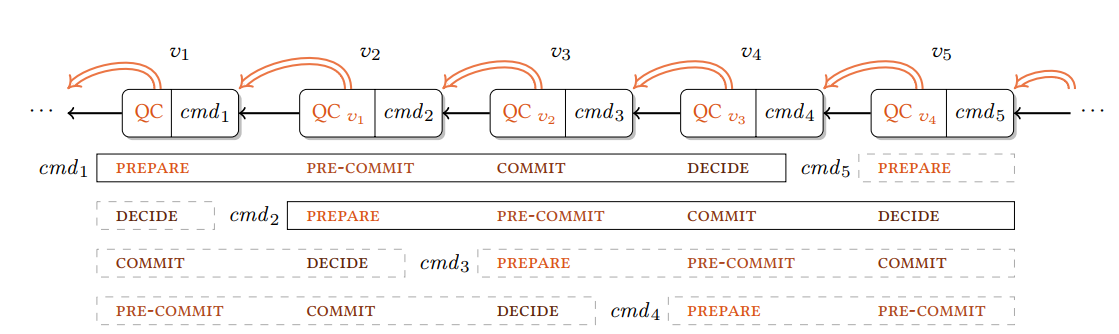
\includegraphics[width=\linewidth]{chained-hotstuff.png}
  \caption{Grund}
  \Description{Grund}
  \label{fig:chained-hotstuff}
\end{figure}

\subsubsection{Angriff auf Chained HotStuff}

To Do


%%
%% Print the bibliography
%%
\printbibliography

\end{document}
\endinput
